\documentclass[a4paper,10pt]{beamer}
\usepackage[utf8]{inputenc}
\usepackage{color}
\usepackage{colortbl}
\usepackage{xcolor}
\usepackage{caption}
\usepackage{enumerate}
\usepackage{ragged2e}
\renewcommand{\figurename}{Figura}
\usetheme{Warsaw}


% !TEX program = pdflatex


\begin{document}

\begin{frame}

 \begin{center}
 \huge{\color{blue}Constraints with Large Scale Structures (Group 1)}
 \end{center}

 \centering
  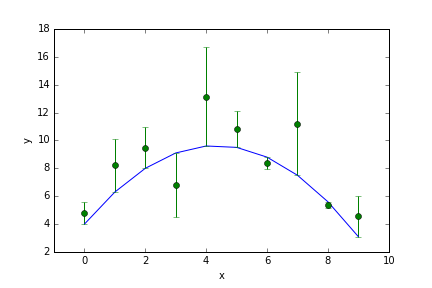
\includegraphics[scale=0.21]{bestfit}
  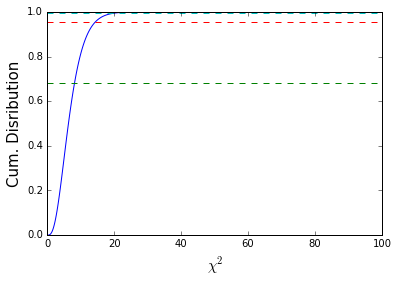
\includegraphics[scale=0.2]{sigmas}
  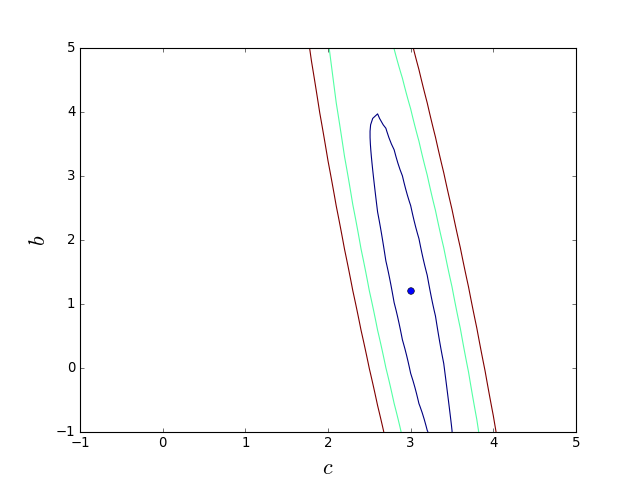
\includegraphics[scale=0.12]{contourcurve}
\begin{columns}[c]
  \column{2.3in}
  \begin{block}{Motivation}
  \begin{itemize}
   \item Learn about the basic tools used to constrain cosmological parameters:
   \begin{enumerate}[(a)]
    \item $\chi^2$ PDF, $\chi^2$ Cumulative Distribution, Confidence levels $\dots$
    \item Programming Language (Python)
    \item Cosmological Tools (CAMB)
   \end{enumerate}
  \end{itemize}
 \end{block}
  \column{2in}
  $\chi^2$ test:
  
  \begin{equation}
   \chi^2 = \sum_{i=1}^n \frac{(y_i^{\text{mod}} - y_i^{\text{data}})^2}{\sigma_i^2}
  \end{equation}

\end{columns}
\end{frame}

\begin{frame}

 \begin{center}
 \huge{\color{blue}CAMB} \\ \large{(Code for Anisotropies in the Microwave Background)} \\
 \vspace{1cm}
 \end{center}
 
 \begin{center}
 \begin{columns}[c]
  \column{2in}
  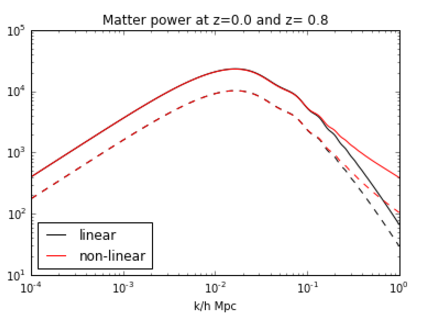
\includegraphics[scale=0.35]{CAMB}
  \column{2in}
  \begin{block}{What have we done so far:}
    \begin{itemize}
     \item Install it!!
     \item Try it (and try to understand it)
    \end{itemize}
  \end{block}

 \end{columns}
 \end{center}
 
 
\end{frame}


\end{document}
